\begin{titlepage}

\newcommand{\HRule}{\rule{\linewidth}{0.5mm}} % Defines a new command for the horizontal lines, change thickness here

\center % Center everything on the page

\begin{minipage}{0.2\textwidth}
\begin{flushleft} \large

\includegraphics[scale=0.3]{epl-logo.jpg}
\end{flushleft}
\end{minipage}
\begin{minipage}{0.6\textwidth}
\begin{flushright} \large
%\textbf{}
\end{flushright}
\end{minipage}\\[0.2cm]
\\
[0.5cm]
{\Large UNIVERSITE CATHOLIQUE DE LOUVAIN-LA-NEUVE}\\[0.1Cm]
%{\huge Rapport de Projet Q4}\\
\\
[0.7cm]
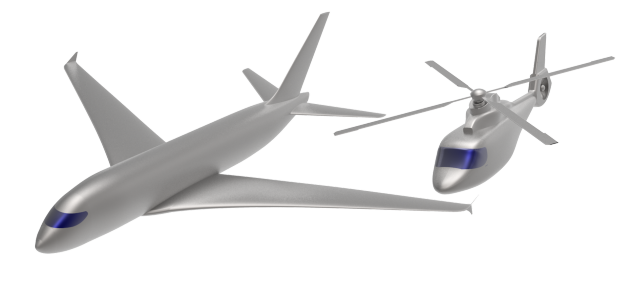
\includegraphics[scale=0.8]{1.png}
\\[1.5cm]
\HRule \\[0.3cm]
{ \huge \textsc{Tuyaux dynamique aérospatiale\\ }}\\[0.25cm] % Title of your document
\HRule \\[3cm]
 
\begin{minipage}{0.4\textwidth}
\begin{flushleft} \large
\emph{\textbf{Auteurs :}}\\

\textsc{De Leener} Maxime\\

\\[0,4cm]
\emph{\textbf{Cours :\ }}\\\textsc{\large LMECA 2830}\\[0.4cm] % Major heading such as course name


\end{flushleft}
\end{minipage}
~
\begin{minipage}{0.4\textwidth}
\begin{flushright} \large
%\emph{\textbf{Coordinateur :}} \\
% \textsc{}\\ [0,5cm] % Supervisor's Name

\emph{\textbf{Professeur :}} \\
\textsc{Chatelain} Philippe\\
\textsc{Schrooyen} Pierre\\ [0,4cm]

\emph{\textbf{Année académique :\ }}\\\textsc{\large 2017-2018}\\[0.4cm] % Minor heading such as course title
%\emph{\textbf{Date de remise :\ }}\\\textsc{\large \textcolor{red}{24 Mars 2017}}\\


\end{flushright}
\end{minipage}\\[0cm]


~
\begin{minipage}{0.4\textwidth}

\end{minipage}

\vfill % Fill the rest of the page with whitespace

\end{titlepage}